  \section{System Design and Architecture}
  \label{sec:system-design}

  In this chapter, the architecture of the system is described. The system is designed to achieve following goals. The system should be modular and easily extensible to allow future extensions towards a full model transformation platform for production use cases. The system should also be maintainable. In the folowing sections, the high-level architecture following the \ac{glsp} architecture is described. Then the design of the components, control flow and data models is described. In the end the UI design is explained.

  \subsection{Following the \ac{glsp} Architecture}
  \label{subsec:high-level-architecture}

  The system is based on the \ac{glsp} architecture, that uses a client-server architecture. The client and server communicate via a websocket connection and JSON-RCP. The \ac{glsp} server can be implemented with Java or Node.js, but due to the constraint that Henshin is implemented in Java, the server is also implemented in Java. The client is implemented in TypeScript. \ac{glsp} provides a defined protocol for the communication between client and server, which can extended with custom commands and actions. The communication is performed using Action Messages, that can be sent from the client and the server to each other or also to itself. The client and the server have Action Handlers, that process the Action Messages and perform the corresponding actions. Each client connection starts its own server instance, therefore each server is only responsible for one client. \cite{glsp-doc} Since each client needs to be able to display three different graph editors for different file types, the server consists of three diagram modules. Each diagram module defines a different diagram language. The \code{XMIDiagramModule} is responsible for the editor of \ac{xmi} instance files, the \code{RuleDiagramModule} is responsible for the editor of Henshin rule files and the \code{EcoreDiagramModule} is responsible for the editor of Ecore metamodel files. In figure \ref{fig:architecture} you can see the high-level architecture of a server and client instance. The architecture of the three diagram modules is quite similar. Each diagram module has a \code{ModelState} which is the central statefull object within a client session \cite{glsp-doc}. The \code{ModelState} is accesed by all other services and handler and represents the current state of the actual source model. \ac{glsp} supports the integration of \ac{emf} models as the underlying source model for the diagrams by default. For that The \code{EMFSourceModelStorage} can load a \ac{emf} file as a \code{RessourceSet}, that is then attached to the \code{ModelState}. That allows an simple integration of the Henshin SDK, since it based on \ac{emf} and provides a \code{HenshinRessourceSet} can be loaded directly over the \ac{emf} integration of \ac{glsp} into the \code{ModelState}.

  The \code{ModelState} of each diagram module also contains an index and a notation model for the layout of the elements in the graphical editor. To be able to have a consistent layout of the elements, not changing after every reload or action, the position and size of each element for each model file is stored in a seperate \textit{.notation} file. The index of the \code{ModelState} is used to map the elements of the source model to the graphical model of \ac{glsp}. For each diagram module, the indexing is implemented in a different way. (see section \ref{subsec:indexing} for more details).

  Another important part of each diagram module is the \code{GModelFactory}, which is responsible for creating the graphical model that is sent to the client from the source model. Since metamodel, transformation and instance \ac{emf} model are strucutred differently, each \code{GModelFactory} of each diagram module is implementing its own mappings.

  \begin{figure}
    \centering
    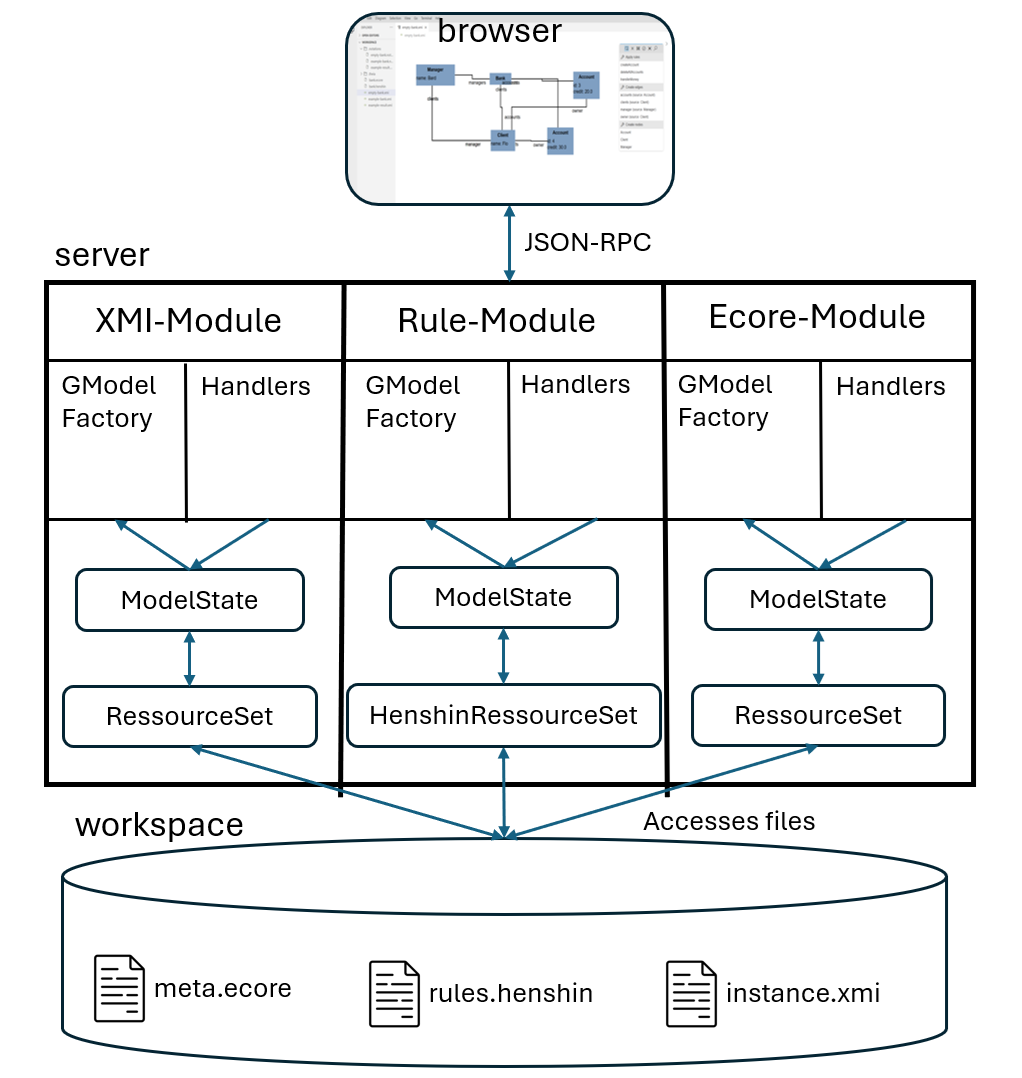
\includegraphics[width=0.6\textwidth]{architecture.png}
    \caption{High-Level Architecture of the System}
    \label{fig:architecture}
  \end{figure}

  \subsection{Data Models and Structures}
  \label{subsec:data-models}

  All three diagram modules have an \ac{emf} based source model. For the Ecore metamodel and the \ac{xmi} instances, The standard data model of \ac{emf} is used. As described in section \ref{subsec:emf} different implementations of \code{EObject} are used, representing all used elements like nodes, attribues or references. For the Hensin transfomations model, the data model of the Henshin \ac{sdk}, that builds upon the \ac{emf} data model, are used. No additional data structures are needed, since every created domain model is based on the \ac{emf} data model. The data model of the graphical representation is provided by \ac{glsp}. It can be extended with custom elements, but the default elements are sufficient for the current use cases. 

  The user has to select or create a workspace in the UI, where all the source models are located. Each workspace for Henshin Web has to be in a specific structure. It should contain one \textit{.ecore} metamodel and one \textit{.henshin} transformations file. Additionally, arbitrary \textit{.xmi} instance files can be added. All of these files should be stored in the root folder of the workspace. When creating a new model file or opening it for the first time, a new notation file is generated and stored in the \textit{.notation} subfolder of the workspace. These notation files are not displayed in the theia explorer.  


  \subsection{Data Flow and Control Flow}
  \label{subsec:data-flow}

  \subsection{Component Design}
  \label{subsec:component-design}

  \subsection{User Interface Design}
  \label{subsec:user-interface-design}

  The design of the user interface is based on the design principles of \ac{glsp} and Eclipse Theia. For editing the graphs, 

  The final UI can be seen in appendix \ref{fig:ecore-ui}, \ref{fig:rule-ui} and \ref{fig:xmi-ui}.

